\documentclass[a4paper]{article}

\usepackage[utf8]{inputenc}
\usepackage[T1]{fontenc}
\usepackage{textcomp}
\usepackage[italian]{babel}
\usepackage{subfig}
\usepackage{amsmath, amssymb}
\usepackage[makeroom]{cancel}
\usepackage{amsfonts}
\usepackage{mdframed}
\usepackage{xcolor}
\usepackage{float}
\usepackage{tikz}
\usepackage{pgfplots}
\usetikzlibrary{pgfplots.fillbetween}
\pgfplotsset{compat=newest, ticks=none}
\usepackage{graphicx}
\graphicspath{{./figures/}}

\pgfdeclarelayer{ft}
\pgfdeclarelayer{bg}
\pgfsetlayers{bg,main,ft}

\usepackage{import}
\usepackage{pdfpages}
\usepackage{transparent}
\usepackage{xcolor}

\usepackage{hyperref}
\hypersetup{
	colorlinks=false,
}

\usepackage{ntheorem}
\newtheorem{theorem}{Teorema}

% Useful definitions frame
\theoremstyle{break}
\theoremheaderfont{\bfseries}
\newmdtheoremenv[%
	linecolor=gray,leftmargin=0,%
	rightmargin=0,
	innertopmargin=8pt,%
	ntheorem]{define}{Definizioni utili}[section]

% Example frame
\theoremstyle{break}
\theoremheaderfont{\bfseries}
\newmdtheoremenv[%
	linecolor=gray,leftmargin=0,%
	rightmargin=0,
	innertopmargin=8pt,%
	ntheorem]{example}{Esempio}[section]

% Important definition frame
\theoremstyle{break}
\theoremheaderfont{\bfseries}
\newmdtheoremenv[%
	linecolor=gray,leftmargin=0,%
	rightmargin=0,
	backgroundcolor=gray!40,%
	innertopmargin=8pt,%
	ntheorem]{definition}{Definizione}[section]

% Exercise frame
\theoremstyle{break}
\theoremheaderfont{\bfseries}
\newmdtheoremenv[%
	linecolor=gray,leftmargin=0,%
	rightmargin=0,
	innertopmargin=8pt,%
	ntheorem]{exercise}{Esercizio}[section]


% figure support
\usepackage{import}
\usepackage{xifthen}
\pdfminorversion=7
\usepackage{pdfpages}
\usepackage{transparent}
\newcommand{\incfig}[1]{%
	\def\svgwidth{\columnwidth}
	\import{./figures/}{#1.pdf_tex}
}

\pdfsuppresswarningpagegroup=1

\begin{document}
\begin{titlepage}
	\begin{center}
		\vspace*{1cm}

		\Huge
		\textbf{Probabilità e Statistica\\Esercizi}

		\vspace{0.5cm}
		\LARGE
		UniVR - Dipartimento di Informatica

		\vspace{1.5cm}

		\textbf{Fabio Irimie}

		\vfill


		\vspace{0.8cm}


		2° Semestre 2023/2024

	\end{center}
\end{titlepage}


\tableofcontents
\pagebreak

% Parte fatta con il prof di esercitazione
\section{Sistema di riferimento}
È un \textbf{sistema di coordinate} rispetto al quale vengono misurate le grandezze coinvolte in un problema.
Per fissare un sistema di riferimento si devono fissare:
\begin{itemize}
	\item Un punto di origine $O$
	\item Un insieme di assi lungo determinate direzioni
\end{itemize}

\subsection{Spazio cartesiano}
È il sistema di riferimento più comune, individuato da 2 o 3 rette mutuamente perpendicolari,
dette \textbf{assi cartesiani}, avendo in comune un unico punto chiamato \textbf{origine}.

\begin{figure}[H]
	\begin{center}
		\begin{tikzpicture}[scale=1.5]
			\draw[->] (-0.2, 0) -- (2, 0) node[right] {$x$};
			\draw[->] (0, -0.2) -- (0, 2) node[above] {$y$};
			\node[below left] at (0,0) {o};

			\draw[dashed] (0,1) -- (1,1) node[right, scale=0.5] {};
			\draw[dashed] (1,0) -- (1,1) node[right, scale=0.5] {};
			\draw[fill] (1,1) circle (0.03) node[above right] {$P(x,y)$};
		\end{tikzpicture}
	\end{center}
	\caption{Spazio cartesiano bidimensionale}
\end{figure}

\begin{definition}[Coordinate cartesiane]
	Le coordinate cartesiane di un punto $P$ nello spazio vengono determinate tracciando il segmento
	di perpendicolare da \( P \) ad ognuno degli assi. La lunghezza di ciascun segmento da \( O \) fino al
	piede della perpendicolare determina il valore della coordinata cartesiana.
\end{definition}
\begin{figure}[H]
	\centering
	\subfloat[Unidimensionale]{%
		\begin{tikzpicture}[scale=0.5,x=0.5cm,y=0.5cm,z=0.3cm,>=stealth]
			\draw[->] (xyz cs:x=-1) -- (xyz cs:x=13.5) node[above] {$x$};

			\node[below] at (0,0,0) {O};
		\end{tikzpicture}
	}%
	\hfill%
	\subfloat[Bidimensionale]{%
		\begin{tikzpicture}[scale=0.5,x=0.5cm,y=0.5cm,z=0.3cm,>=stealth]
			\draw[->] (xyz cs:x=-1) -- (xyz cs:x=13.5) node[above] {$x$};
			\draw[->] (xyz cs:y=-1) -- (xyz cs:y=13.5) node[right] {$z$};

			\node[below right] at (0,0,0) {O};
		\end{tikzpicture}
	}%
	%
	\subfloat[Tridimensionale]{%
		\begin{tikzpicture}[scale=0.5,x=0.5cm,y=0.5cm,z=0.3cm,>=stealth]
			% The axes
			\draw[->] (xyz cs:x=-1) -- (xyz cs:x=13.5) node[above] {$x$};
			\draw[->] (xyz cs:y=-1) -- (xyz cs:y=13.5) node[right] {$z$};
			\draw[->] (xyz cs:z=-1) -- (xyz cs:z=13.5) node[above] {$y$};

			\node[below right] at (0,0,0) {O};
		\end{tikzpicture}
	}%
	\caption{Tipi di spazio cartesiano}
\end{figure}

\section{Grandezze}
\subsection{Grandezze scalari}
Sono grandezze che si possono rappresentare con un numero reale, ad esempio la massa, la temperatura, ecc.
Per definire una grandezza scalare è necessario specificare:
\begin{itemize}
	\item Il valore numerico
	\item L'unità di misura
\end{itemize}

\subsection{Grandezze vettoriali}
Sono grandezze che si possono rappresentare con un \textbf{vettore}, ad esempio la forza, la velocità, ecc.
Per definire una grandezza vettoriale è necessario utilizzare un vettore, cioè un segmento orientato
definito da:
\begin{itemize}
	\item Intensità (o modulo)
	\item Direzione
	\item Verso
\end{itemize}

\begin{figure}[H]
	\centering
	\begin{tikzpicture}
		\draw[->, thick] (0,0) -- (2,0) node[above] {verso};
		\draw[dashed] (-5,0) -- (0,0);
		\draw[dashed] (2,0) -- (5,0) node[right] {direzione};

		\draw (0,-0.2) -- ++(0,-0.2) -- ++(2,0) -- ++(0,0.2);
		\node[below, yshift=-5] at (1,-0.2) {intensità};
	\end{tikzpicture}
	\caption{Rappresentazione di un vettore}
\end{figure}

\noindent Si può moltiplicare un vettore per uno scalare, ottenendo un vettore con direzione del primo vettore
e intensità uguale al prodotto del modulo del primo vettore per lo scalare. Il verso resterà lo stesso
del primo vettore in caso di scalare positivo e sarà opposto in caso di scalare negativo.

\subsubsection{Scomposizione di un vettore}
Un vettore può essere scomposto in due vettori, detti \textbf{componenti}, lungo due direzioni ortogonali.
\[
	\vec{v} = \vec{v_x} + \vec{v_y} \quad \text{\textbf{somma vettoriale}}
\]
\begin{figure}[H]
	\centering
	\begin{tikzpicture}[scale=2]
		\draw[->] (-0.2, 0) -- (2, 0) node[right] {$x$};
		\draw[->] (0, -0.2) -- (0, 2) node[above] {$y$};
		\node[below left] at (0,0) {o};

		\draw[->, thick, blue] (0,0) -- (1.2,1.2);
		\draw (0.5,0) arc (0:45:0.5) node[below right, xshift=5] {$\alpha$};
		\draw[dashed] (1.2,1.2) -- (1.2,0);
		\draw[dashed] (1.2,1.2) -- (0,1.2);

		\node[left, xshift=-5, blue] at (0.8,0.8) {$\vec{v}$};

		\draw[->, thick, red] (0,0) -- (1.2,0) node[below] {$\vec{v_x}$};
		\draw[->, thick, red] (0,0) -- (0,1.2) node[left] {$\vec{v_y}$};
	\end{tikzpicture}
	\caption{Scomposizione di un vettore}
\end{figure}

\noindent Il modulo del vettore \( \vec{v} \) si trova applicando il teorema di Pitagora al modulo delle componenti:
\[
	|\vec{v}| = \sqrt{|\vec{v_x}|^2 + |\vec{v_y}|^2}
\]
\subsubsection{Versori}
Sono \textbf{vettori unitari} (con \( modulo=1 \)) diretti come gli assi, in genere indicati come
\( \hat{i},\hat{j},\hat{k} \).

\noindent Un vettore può essere indicato come somma dei versori, ciascuno moltiplicato per il modulo
della rispettiva componente del vettore:
\[
	\vec{v} = v_x\hat{i} + v_y\hat{j}
\]
Ad esempio:
\[
	\vec{a} = 2\hat{i} + 3\hat{j} \quad \text{o} \;\; \vec{a}(2,3)
\]

\subsubsection{Somma di vettori}
La somma di due vettori si ottiene sommando le rispettive componenti:
\begin{figure}[H]
	\centering
	\begin{tikzpicture}[scale=2]
		\draw[->] (-0.2, 0) -- (2, 0) node[right] {$x$};
		\draw[->] (0, -0.2) -- (0, 2) node[above] {$y$};
		\node[below left] at (0,0) {o};

		\draw[->, thick, blue] (0,0) -- (1.5,1.6);

		\draw[->, thick, red] (0,0) -- (1,0.5);
		\draw[->, thick, red] (1,0.5) -- (1.5,1.6);

		\node[left, xshift=-5, blue] at (0.8,0.8) {$\vec{C}$};
		\node[left, xshift=-5, red] at (0.8,0.18) {$\vec{A}$};
		\node[left, xshift=-5, red] at (1.6,1.05) {$\vec{B}$};
	\end{tikzpicture}
	\caption{Somma di vettori}
\end{figure}
\[
	\vec{C} = \vec{A} + \vec{B}
\]
\[
	A_x+B_x = C_x \quad A_y+B_y = C_y
\]
\[
	\vec{C} = C_x\hat{i} + C_y\hat{j}
\]

\subsubsection{Differenza di vettori}
La differenza di due vettori si ottiene sottraendo le rispettive componenti:
\begin{figure}[H]
	\centering
	\begin{tikzpicture}[scale=2]
		\draw[->] (-0.2, 0) -- (1.7, 0) node[right] {$x$};
		\draw[->] (0, -0.2) -- (0, 1.7) node[above] {$y$};
		\node[below left] at (0,0) {o};

		\draw[->, thick, blue] (0.5,1) -- (1,0.3) node[above, yshift=5] {$\vec{C}$};

		\draw[->, thick, red] (0,0) -- (0.99,0.29) node[below] {$\vec{A}$};
		\draw[->, thick, red] (0,0) -- (0.49,0.99) node[left] {$\vec{B}$};
	\end{tikzpicture}
	\caption{Differenza di vettori}
\end{figure}
\[
	\vec{C} = \vec{A} - \vec{B} = \vec{A} + (-\vec{B})
\]
\[
	A_x-B_x = C_x \quad A_y-B_y = C_y
\]
\[
	\vec{C} = C_x\hat{i} + C_y\hat{j}
\]

\subsection{Rapporti trigonometrici}
\[
	\sin(\alpha) = \frac{opposto}{ipotenusa}
\]
\[
	\cos(\alpha) = \frac{adiacente}{ipotenusa}
\]
\[
	\tan(\alpha) = \frac{opposto}{adiacente}
\]

\subsection{Prodotto scalare}
Il prodotto scalare tra due vettori \( \vec{A} \) e \( \vec{B} \) è definito come:
\[
	\vec{A} \cdot \vec{B} = AB\cos(\alpha)
\]
Dove \( \alpha \) è l'angolo tra i due vettori.
\[
	\alpha = 0 \quad A \cdot B = AB
\]
\[
	\alpha = 90\quad A \cdot B = 0
\]
\[
	\alpha = 180\quad A \cdot B = -AB
\]
Il prodotto scalare è quindi il numero che si ottiene moltiplicando il modulo del primo per
l'intensità del vettore componente del secondo lungo il primo (\( b \cos{\alpha} \)). Un altro modo per scriverlo è:
\[
	\vec{a} \cdot \vec{b} = ab\cos(\alpha) = ab_a
\]
Dove \( b_a = b\cos(\alpha) \)

\subsubsection{Prodotto scalare tramite componenti}
Presi 2 vettori:
\[
	\vec{A} = a_x\hat{i} + a_y\hat{j} + a_z\hat{k} \quad \vec{A}(a_x,a_y,a_z)
\]
\[
	\vec{B} = b_x\hat{i} + b_y\hat{j} + b_z\hat{k} \quad \vec{B}(b_x,b_y,b_z)
\]
Il prodotto scalare si può calcolare come:
\[
	C = \vec{A} \cdot \vec{B} = a_xb_x + a_yb_y + a_zb_z
\]
Perchè:
\[
	\hat{i} \cdot \hat{i} = \hat{j} \cdot \hat{j} = \hat{k} \cdot \hat{k} = 1
\]
\[
	\hat{i} \cdot \hat{j} = \hat{i} \cdot \hat{k} = \hat{j} \cdot \hat{k} = 0
\]

\begin{figure}[H]
	\begin{example}
		\[
			\vec{A} = 3\hat{i} + 2\hat{j} \quad \vec{B} = \hat{i} + 2\hat{j}
		\]
		\[
			\vec{A} \cdot \vec{B} = 2\cdot3 + 3\cdot4 = 6 + 12 = 18
		\]
		\[
			C = \vec{A} \cdot \vec{B} = (3\hat{i} + 2\hat{j}) \cdot (\hat{i} + 2\hat{j}) = 3\cdot1 + 2\cdot2 = 3 + 4 = 7
		\]
	\end{example}
\end{figure}

\subsection{Prodotto vettoriale}
Il prodotto vettoriale tra 2 vettori, è un vettore avente modulo uguale al prodotto dei loro
moduli per il seno dell'angolo compreso tra essi:
\[
	|\vec{a} \times \vec{b}| = ab \sin(\alpha)
\]
La direzione si individuano con la regola della mano destra.

\begin{figure}[H]
	\centering
	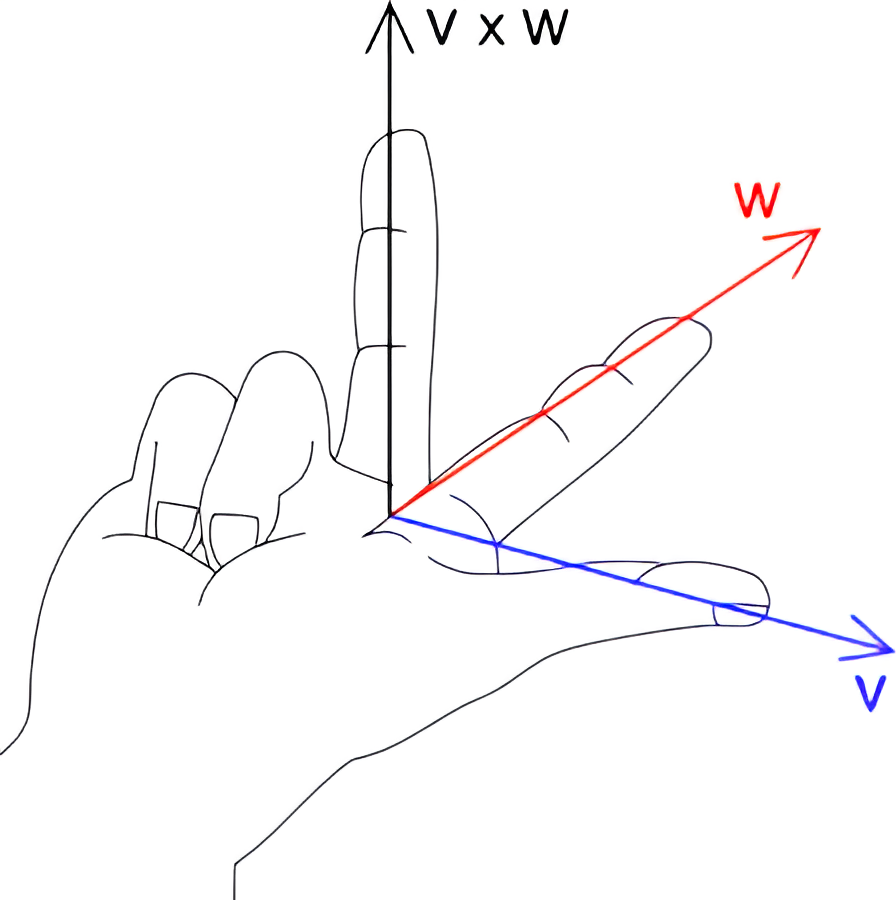
\includegraphics[width=0.4\textwidth]{manoDestra}
	\caption{Regola della mano destra}
\end{figure}

\noindent Il modulo del vettore risultante è uguale all'area del parallelogramma generato dai vettori \( \vec{a} \) e \( \vec{b} \).

% Prof di teoria
\section{Moto in una dimensione}
\subsection{Posizion, distanza e spostamento}

\subsection{Velocità}
\subsubsection{Velocità media}
\begin{definition}[Velocità media]
	La velocità media di un corpo è definita come il rapporto tra lo spostamento e l'intervallo di tempo
	\[
		\bar{v} = \frac{\Delta s}{\Delta t} \; \left[ \frac{m}{s} \right]
	\]
\end{definition}

Se la velocità è:
\begin{itemize}
	\item \( v > 0 \) il corpo si muove in direzione positiva
	\item \( v < 0 \) il corpo si muove in direzione negativa
\end{itemize}

\subsubsection{Velocità istantanea}
\begin{definition}[Velocità istantanea]
	La velocità istantanea di un corpo è definita come il limite della velocità media
	per intervalli di tempo sempre più piccoli
	\[
		v = \lim_{\Delta t \to 0} \frac{\Delta s}{\Delta t} = \frac{ds}{dt}
	\]
\end{definition}

Se la velocità istantanea è:
\begin{itemize}
	\item \( v > 0 \) il corpo si muove in direzione positiva
	\item \( v < 0 \) il corpo si muove in direzione negativa
	\item \( v = costante \) il corpo si muove con moto rettilineo uniforme e la sua funzione è:
    \[
    s(t) = s_0 + v_0t
    \] 
\end{itemize}

\subsection{Accelerazione}
\subsubsection{Accelerazione media}
\begin{definition}[Accelerazione media]
  L'accelerazione media di un corpo è definita come il rapporto tra la variazione di velocità e l'intervallo di tempo
  \[
    \bar{a} = \frac{\Delta v}{\Delta t} \; \left[ \frac{m}{s^2} \right]
  \]
\end{definition}

\end{document}
